%% @Author: Ines Abdeljaoued Tej
%  @Date:   2018-06
%% @Class:  Graduation Project, ESSAI - Carthage University, Tunisia.

\documentclass[a4paper, oneside, french, 12pt, final]{extreport}
\usepackage[utf8]{inputenc}

\parindent 0cm
\usepackage{makeidx}
\makeindex

\usepackage[lined,boxed,commentsnumbered, ruled,vlined,linesnumbered]{algorithm2e}
\usepackage{amsthm}
\newtheorem{theorem}{Theorem}[chapter]
\newtheorem{definition}{Definition}[chapter]
\newtheorem{exemple}{Example}[chapter]


%\usepackage[nottoc]{tocbibind}
%\addcontentsline{toc}{section}{References}

\providecommand{\keywords}[1]{\textbf{\textit{Keywords---}} #1}

\usepackage{etoolbox}
%\makeatletter
%\patchcmd{\thebibliography}{%
%  \chapter*{\bibname}\@mkboth{\MakeUppercase\bibname}%{\MakeUppercase\bibname}}{%
%  \section{References}}{}{}
%\makeatother

\usepackage[utf8]{inputenc}
\usepackage[english]{babel}

\usepackage[nottoc]{tocbibind}

\textwidth 18cm
\textheight 24cm
\topmargin -0.5cm
\oddsidemargin -1cm

% set font encoding for PDFLaTeX or XeLaTeX
\usepackage{ifxetex}
\ifxetex
  \usepackage{fontspec}
\else
  \usepackage[T1]{fontenc}
  \usepackage[utf8]{inputenc}
  \usepackage{lmodern}
\fi


% Enable SageTeX to run SageMath code right inside this LaTeX file.
% documentation: http://mirrors.ctan.org/macros/latex/contrib/sagetex/sagetexpackage.pdf
%\usepackage{sagetex}


\newcommand{\reportTitle} {%
  \textsc{Graduation Project Report}
  %\textsc{Projet de Fin d'\'etudes}
}

\newcommand{\reportAuthor} {%
  FirstName \textsc{LastName}%
}

\newcommand{\reportSubject} {%
  My very attractive \\ Title%
}

\newcommand{\dateSoutenance} {%
  12/06/2018%
}

\newcommand{\studyDepartment} {%
  Entreprise d'accueil %Statistique
}

\newcommand{\ESSAI} {%
  Higher School of Statistics and Information Analysis
  %Ecole Sup\'erieure de la Statistique et de l'Analyse de l'Information
}

%\newcommand{\codePFE} {% Reference
%  Code PFE%
%}

\newcommand{\juryPresident} {%
  Mr Ben Foulen \textsc{Foulenia}%
}
\newcommand{\juryPresidentDesc} {%
  President%
}

\newcommand{\juryMemberOne} {%
  Ms Ben Foulena \textsc{Foulen}%
}
\newcommand{\juryMemberOneDesc} {%
  Examiner %Mentor
}

\newcommand{\juryMemberTwo} {%
  Mr Ben Foulen \textsc{Fouleni}%
}
\newcommand{\juryMemberTwoDesc} {%
  Reviewer% Examiner, Reporter
}

\newcommand{\juryMemberThree} {%
	M. Ben Foulen \textsc{Fouleni}%
}
\newcommand{\juryMemberThreeDesc} {%
	Supervisor% Examiner, Reporter
}

\newcommand{\juryMemberFour} {%
	M. Ben Foulen \textsc{Fouleni}%
}
\newcommand{\juryMemberFourDesc} {%
	Mentor% Examiner, Reporter
}


\newcommand{\specialcell}[1]{%
  \begin{tabularx}{\textwidth}{@{}X@{}}#1\end{tabularx}%
}

%%%%%%%%%%%%%%%%%%%%%%%%%%%%%%%%%%%%%%%%%%%%%%%%%%%%%%%
% Add your own commands here
%%%%%%%%%%%%%%%%%%%%%%%%%%%%%%%%%%%%%%%%%%%%%%%%%%%%%%%
\newcommand{\MyCommand} {%
  Does nothing really%
}


% used in maketitle
\title{\reportSubject}
\author{\reportAuthor}

% Enable SageTeX to run SageMath code right inside this LaTeX file.
% documentation: http://mirrors.ctan.org/macros/latex/contrib/sagetex/sagetexpackage.pdf
%\usepackage{sagetex}

%\hypersetup{
%  pdftitle={\reportTitle~-~\reportSubject},%
%  pdfauthor={\reportAuthor},%
%  pdfsubject={\reportSubject},%
%  pdfkeywords={report} {internship} {pfe} {enis}
%}

\usepackage{graphics}
\usepackage{graphicx}


\usepackage[acronym,toc,section=chapter]{glossaries}
\makeglossaries

\newacronym{abc}{ABC}{A contrived acronym}
\newacronym{efg}{EFG}{Another acronym}
\newacronym{svm}{SVM}{Support Vector Machines}

\pagenumbering{roman}
\begin{document}

\thispagestyle{empty}
\begin{titlepage}
\begin{center}


%%%%%%%%%%%%%%%%%%%%%%%%%%%%%%%%%%%%%%%%%%%%%%%
% THE HEADER
%%%%%%%%%%%%%%%%%%%%%%%%%%%%%%%%%%%%%%%%%%%%%%%

\includegraphics[width=2cm, height=1.5cm]{embleme.jpg}\\

{%
  \fontsize{9pt}{9pt}\selectfont%
  \begin{tabular}{c}
    Tunisian Republic\\
    Ministry of Higher Education and Scientific Research \\%
    Carthage University - \ESSAI{}  \\
    % Column 2
    %\studyDepartment \\
    % Engineering Education Computer Engineering and Applied Mathematics Discipline%
    % Cycle de Formation d'Ing\'enieurs en  Statistique et Analyse de l'Information%
    %Carthage University
  \end{tabular}
}

\vspace{10pt}

\includegraphics[width=4cm, height=2.5cm]{universite-carthage.jpg} \\

%%%%%%%%%%%%%%%%%%%%%%%%%%%%%%%%%%%%%%%%%%%%%%%
% THE PAGE CONTENT
%%%%%%%%%%%%%%%%%%%%%%%%%%%%%%%%%%%%%%%%%%%%%%%

\vspace{10pt} {%
  \renewcommand*{\familydefault}{\defaultFont}
  \fontsize{46pt}{46pt}\selectfont%
  % MEMOIRE\\%
  %\reportTitle{}%\\\textsc{Report}\\%
}

\vspace{10pt}
\textbf{\textit{Graduation Project Report submitted in partial fulfillment of}}\\
\textbf{\textit{the requirements for the degree of}}\\

\vspace{10pt}
Engineering Diploma in Statistics and Data Analysis\\


\includegraphics[width=2.5cm, height=2.5cm]{logo-essai.jpg}\\

\vspace{10pt}
\textbf{\textit{Submitted by}}\\
\vspace{10pt} {%
  \fontsize{18pt}{18pt}\selectfont%
  \textbf{\reportAuthor}\\
}%

\vspace{10pt} {%
  \renewcommand*{\familydefault}{\defaultFont}
  \fontsize{27pt}{27pt}\selectfont%
  \rule{0.5\textwidth}{.4pt}\\
  \vspace{10pt}
  \reportSubject{}\\%
  \vspace{10pt}
  \rule{0.5\textwidth}{.4pt}
}

\vspace{10pt}
Defended on~\dateSoutenance~ in front of the committee composed of:\\
%Soutenu le \dateSoutenance, devant la commission d'examen:\\
\vspace{20pt}
\begin{tabular}{p{0.3\linewidth} p{0.15\linewidth}}
  \juryPresident{} & \juryPresidentDesc{}\\
  \juryMemberOne{} & \juryMemberOneDesc{}\\
  \juryMemberTwo{} & \juryMemberTwoDesc{}\\
  \juryMemberThree{} & \juryMemberThreeDesc{}\\
  \juryMemberFour{} & \juryMemberFourDesc{}\\
\end{tabular}

\vspace{10pt}%
\textbf{\textit{A Graduation Project made at}}\\

\vspace{10pt}
(\studyDepartment)\\

\end{center}
\end{titlepage}

%\begin{pfe-essai}
%%%%%%%%%%%%%%%%%%%%%%%%%%%%%%%%%%%%%%%%%%%%%%%%%%%%%%%
% Table des matières, figures, tableaux ; Glossaire
%%%%%%%%%%%%%%%%%%%%%%%%%%%%%%%%%%%%%%%%%%%%%%%%%%%%%%%



% ###############################
% # HELP COMMANDS               #
% ###############################
%
% -1 \part{part}
%  0 \chapter{chapter}
%  1 \section{section}
%  2 \subsection{subsection}
%  3 \subsubsection{subsubsection}
%  4 \paragraph{paragraph}
%  5 \subparagraph{subparagraph}


%%%%%%%%%%%%%%%%%%%%%%%%%%%%%%%%%%%%%%%%%%%%%%%%%%%%%%%
% Dédicace et Remerciements
%%%%%%%%%%%%%%%%%%%%%%%%%%%%%%%%%%%%%%%%%%%%%%%%%%%%%%%
	

%\printglossary[type=abbrev]



\chapter*{Dedication}
%\chapter*{D\'edicace}
%\addcontentsline{toc}{chapter}{Dedication}
\thispagestyle{empty}
%
%For all they have endured to satisfy all my needs and wishes

\begin{center}
 {\it 
	
A ... pour son(leur) sacrifice et son(leur) soutien, \\
en témoignage de mon infinie reconnaissance et mon profond attachement \\
\vspace{1cm}
A tous ceux qui me sont chers...

}
\end{center}
%
%\nopagebreak{%
% And maybe a quote here
% \raggedright\hspace{5.75cm} To all of you,~\\
%\raggedright\hspace{7.75cm} I dedicate this work.
%  \raggedleft\normalfont\large\itshape{} \reportAuthor\par%
%}
%
%\cleardoublepage%

\chapter*{Thanks}
%\chapter*{Remerciements}
%\addcontentsline{toc}{chapter}{Thanks}
\thispagestyle{empty}

Je n'aurais jamais pu réaliser ce projet sans la précieuse aide et sans le soutien d'un grand nombre de personnes ... En premier lieu, je tiens à remercier mon encadrant universitaire, \juryMemberFour{}, pour . Je souhaiterais exprimer ma gratitude à \juryMemberThree{}, pour m’avoir donné envie de réaliser un mémoire sur ... au sein de \studyDepartment. Je le remercie également pour son accueil... J'aimerais également dire à \juryPresident{} à quel point je suis honorée. Je suis infiniment gré à (Mme, M.) \juryMemberOne{} de s’être rendu(e) disponible, je suis particulièrement reconnaissant(e) à \juryMemberTwo{} de l’intérêt qu’il a manifesté à l’égard de ce projet en s’engageant à être rapporteur. \\

Ma reconnaissance va à ceux qui ont plus particulièrement assuré le soutien affectif de ce travail : ma famille ainsi que mes amis. 

\tableofcontents
\addcontentsline{toc}{chapter}{\contentsname}
\cleardoublepage%

\listoffigures
%\addcontentsline{toc}{chapter}{\listfigurename}
\cleardoublepage%

\listoftables
%\addcontentsline{toc}{chapter}{\listtablename}
\cleardoublepage

\listofalgorithms
\addcontentsline{toc}{chapter}{List of Algorithms}
\cleardoublepage
    %\printacronyms[heading=chapter*, name=Acronyms]
    %\printacronyms[heading=chapter*, name=Notations]
    


    %\sloppy

    \pagenumbering{arabic}% 1 2 3 4 5
%    \doublespacing{}% Double spacing between lines

    \addtocontents{toc}{\protect\setcounter{tocdepth}{2}}


%%%%%%%%%%%%%%%%%%%%%%%%%%%%%%%%%%%%%%%%%%%%%%%%%%%%%%%
% Divers chapitres
%%%%%%%%%%%%%%%%%%%%%%%%%%%%%%%%%%%%%%%%%%%%%%%%%%%%%%%

\pagenumbering{arabic}

\chapter*{Introduction}
\label{chap:general_intorduction}
\markboth{\MakeUppercase{Introduction}}{}%
%\addcontentsline{toc}{chapter}{Introduction}%

%% @Author: Ines Abdeljaoued Tej
%  @Date:   2018-06
%% @Class:  PFE de l'ESSAI - Universite de Carthage, Tunisie.


\markboth{\MakeUppercase{Introduction}}{}%
\addcontentsline{toc}{chapter}{Introduction}%

%Welcome to \Ac{ESSAI}. ~\\
%Again, welcome to \Ac{ESSAI}. ~\\
%Your introduction goes here. ~\\

Voici une référence à l'image de la Figure \ref{fig:test} page \pageref{fig:test} et une autre vers la partie \ref{chap:2} page \pageref{chap:2}.
On peut citer un livre\, \cite{caillois1} et on précise les détails à la fin du rapport dans la partie références.
Voici une note\,\footnote{Texte de bas de page} de bas de page\footnote{J'ai bien dit bas de page}. Nous pouvons également citer l'Algorithme \ref{algo1}, la Définition \ref{def1}, le Théorème \ref{theo1} ou l'Exemple \ref{exo1}...\\

Le document est déatillé comme suit : le chapitre \ref{chap:chapterone} introduit le cadre général de ce travail. Il s'agit de présenter l'entreprise d'accueil et de détailler la problématique. Le chapitre \ref{chap:2} introduit les données ainsi que les modèles choisies. Le chapitre \ref{chap:3} donne les principaux résultats et la comparaison entre divers modèles (courbe de ROC, indice de Gini). Nous clôturons ce travail par une brève conclusion résumant le travail accompli ainsi que des perspectives qui pourraient enrichir ce travail.  




\chapter{Chapter One}%
\label{chap:chapterone}

%% @Author: Ines Abdeljaoued Tej
%  @Date:   2018-06
%% @Class:  PFE de l'ESSAI - Universite de Carthage, Tunisie.

%%%%%%%%%%%%%%%%%%%%%%%%%%%%
% SECTION                  %
%%%%%%%%%%%%%%%%%%%%%%%%%%%%
\section{Section une}
\label{chap:sectionone}

\subsection{Sub section One}

And your chapter one goes here \cite{web001,Nom2012}. \\
  Lorem ipsum dolor sit amet, consectetur adipisicing elit, sed do eiusmod
  tempor incididunt ut labore et dolore magna aliqua. Ut enim ad minim veniam, quis nostrud exercitation ullamco laboris nisi ut aliquip ex ea commodo consequat. Duis aute irure dolor in reprehenderit in voluptate velit esse \cite{Bird02nltk:the}
  cillum dolore eu fugiat nulla pariatur. Excepteur sint occaecat cupidatat non
  proident, sunt in culpa qui officia deserunt mollit anim id est laborum.

  \begin{figure}[h]%
    \center%
    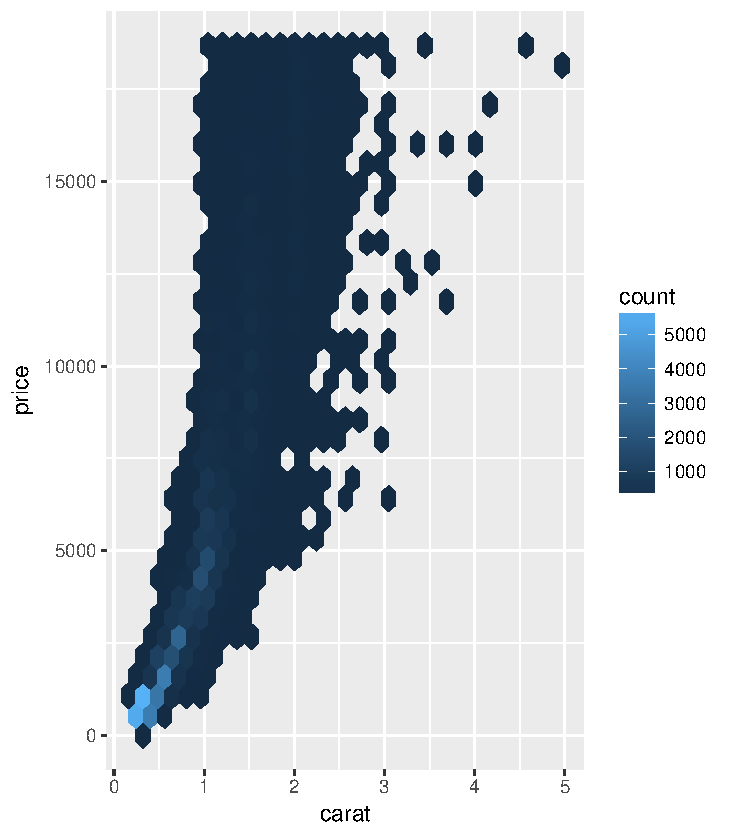
\includegraphics[width=0.3\textwidth]{diamonds.pdf}
    \caption[This is a test image]{Test Image}\label{fig:test}%
  \end{figure}


\begin{table}\begin{center}
\begin{tabular}{c|c}
Entrée & Sortie \\ \hline 
A & B \\
C & D
\end{tabular}
\caption{Test Table}\end{center}
\end{table}


\subsection{Sub section Two}

  This is a second subsection\cite{gen1972}, \cite{schaeffer99}. ~\\
  Lorem ipsum dolor sit amet, consectetur adipisicing elit, sed do eiusmod
  tempor incididunt ut labore et dolore magna aliqua. Ut enim ad minim veniam,
  quis nostrud exercitation ullamco laboris nisi ut aliquip ex ea commodo
  consequat. Duis aute irure dolor in reprehenderit in voluptate velit esse
  cillum dolore eu fugiat nulla pariatur. Excepteur sint occaecat cupidatat non
  proident, sunt in culpa qui officia deserunt mollit anim id est laborum.

  \begin{description}\addtolength{\itemsep}{-0.35\baselineskip}%
    \item[\textbullet~\bfseries Menu Item] \hfill \\%
      Menu Description.~\\%
      {\textbf{Focus topics:~}\emph{Topic one, topic two, topic three, ...}}%
    %
    \item[\textbullet~\bfseries Menu Item] \hfill \\%
      Menu Description.~\\%
      {\textbf{Focus topics:~}\emph{Topic one, topic two, topic three, ...}}%
    %
    \item[\textbullet~\bfseries Menu Item] \hfill \\%
      Menu Description.~\\%
      {\textbf{Focus topics:~}\emph{Topic one, topic two, topic three, ...}}%
  \end{description}

  Also bullets such as:%
  \begin{itemize}\addtolength{\itemsep}{-0.35\baselineskip}%
    \item One%
    \item Two%
    \item Three%
    \item Four%
    \item \ldots%
  \end{itemize}%
  %
\section{powers series} \label{subsection}

\begin{equation} \label{eq:1}
\sum_{i=0}^{\infty} a_i x^i
\end{equation}

The equation \ref{eq:1} is a typical power series.

\chapter{Modelling data}
\label{chap:2}
%% @Author: Ines Abdeljaoued Tej
%  @Date:   2018-06
%% @Class:  Graduation Project, ESSAI - Carthage University, Tunisia.
  

\begin{itemize}
	\item The individual \index{Entries}{entries} are indicated with a black dot, a so-called bullet.
	\item The text in the entries may be of any length.
\end{itemize}

\begin{theorem}\label{theo1}
Soit $n$ un entier naturel. Si $n$ est premier alors il n'est divisible que par 1 et par lui-même.
\end{theorem}

\begin{proof}
Here is my proof.
\end{proof}

\begin{definition}\label{def1}
Soit $A$ une courbe...
\end{definition}

Ici, il s'agit de l'utilisation de TB %\nomenclature[TB]{TB}{Très Bien} qui consiste à parler Très Bien. 
\gls{abc} et \gls{efg} sont des acronyms et des abbréviations... La méthode \gls{svm} est également couramment utilisée.

\begin{exemple}\label{exo1}
On considère le cas particulier... 
\end{exemple}

\chapter{Results}
\label{chap:3}
\markboth{\MakeUppercase{Autrechap}}{}%
\addcontentsline{toc}{chapter}{Autre Chapitre}%
%% @Author: Ines Abdeljaoued Tej
%  @Date:   2018-06
%% @Class:  Graduation Project, ESSAI - Carthage University, Tunisia.


Exemple d'un algorithme : \\

\begin{algorithm}[H]
\DontPrintSemicolon
\SetAlgoLined
%\KwResult{Write here the result}
\SetKwInOut{Input}{Input}\SetKwInOut{Output}{Output}
\Input{Write here the input}
\Output{Write here the output}
\BlankLine
 
\While{While condition}{
    instructions\;
    \eIf{condition}{
        instructions1\;
        instructions2\;
    }{
        instructions3\;
    }
}
\caption{While loop with If/Else condition}\label{algo1}
\end{algorithm}



\begin{algorithm}[H]
\DontPrintSemicolon
\SetAlgoLined
%\KwResult{Write here the result}
\SetKwInOut{Input}{Entrée}\SetKwInOut{Output}{Sortie}
\Input{Write here the input}
\Output{Write here the output}
\BlankLine
 
$x\leftarrow 0$    \;
$y\leftarrow 0$    \;
\BlankLine
\ForEach{ForEach condition}{    
    
    \BlankLine
    
    \tcc{comments on code}    
    \ForEach{ForEach condition}{
        \If{If condition}{
            instruction(s) like below: \\
            increase $x$ by $1$\;
            decrease $y$ by $2$\;
        }
                
        \BlankLine
        
        \uIf{If condition}{
            instruction
        }
        \uElseIf{ElseIf condition}{
            instruction
        }
        \uElse{
            instruction
        }                
    }    
}
\caption{Nested ForEach loop with If/ElseIf/Else condition}
\end{algorithm}


\chapter*{Conclusion}
\label{chap:conclusion}
\markboth{\MakeUppercase{Conclusion}}{}%
\addcontentsline{toc}{chapter}{Conclusion}
  And a very interesting conclusion here\@. ~\\
  Lorem ipsum dolor sit amet, consectetur adipisicing elit, sed do eiusmod
  tempor incididunt ut labore et dolore magna aliqua. Ut enim ad minim veniam,
  quis nostrud exercitation ullamco laboris nisi ut aliquip ex ea commodo
  consequat.

\newpage
\appendix
\addcontentsline{toc}{chapter}{Appendix}
%\markboth{\MakeUppercase{Annexe}}{}

\chapter{Code R pour résoudre la problématique}
\label{chap:appendix}


\section{Pré-traitement des données}
\section{Code R pour les modèles}

\chapter{Code Python pour résoudre la problématique}
\label{chap:appendixB}
\section{Tests avec le package {\tt Numpy}}

 An appedix if you need it.
 
 \begin{verbatim}
 Insérer ici le code !
 \end{verbatim}

\section{Librairies utilisées}
 
  Lorem ipsum dolor sit amet, consectetur adipisicing elit, sed do eiusmod
  tempor incididunt ut labore et dolore magna aliqua. Ut enim ad minim veniam,
  quis nostrud exercitation ullamco laboris nisi ut aliquip ex ea commodo.



\bibliographystyle{apalike}
\bibliography{Biblio}

\cleardoublepage%

\addtocontents{toc}{\protect\setcounter{tocdepth}{3}}

\printglossaries
\printindex

\begin{abstract}

Put here an absract for the report; \\

\keywords{Insert 5 keywords}
\end{abstract}

\end{document}